\documentclass[conference]{IEEEtran}
\IEEEoverridecommandlockouts

\usepackage{cite}
\usepackage{amsmath,amssymb,amsfonts}
\usepackage{algorithmic}
\usepackage{graphicx}
\usepackage{textcomp}
\usepackage{xcolor}

\def\BibTeX{{\rm B\kern-.05em{\sc i\kern-.025em b}\kern-.08em
    T\kern-.1667em\lower.7ex\hbox{E}\kern-.125emX}}
    
% A shortcut for µRTS
\newcommand{\mRTS}{$\mu$RTS}

\begin{document}

\title{Enhancing MCTS Performance in Real-Time Strategy Games Through Move Pruning}

\author{
\IEEEauthorblockN{Abdessamed Ouessai\IEEEauthorrefmark{1}, Mohammed Salem\IEEEauthorrefmark{1} and Antonio M. Mora\IEEEauthorrefmark{2}}

\IEEEauthorblockA{\IEEEauthorrefmark{1}Dept. of Computer Sciences, University of Mascara, Algeria.\\
abdessamed.ouessai@univ-mascara.dz, salem@univ-mascara.dz}

\IEEEauthorblockA{\IEEEauthorrefmark{2}Dept. of Signal Theory, Telematics and Communications, ETSIIT-CITIC, University of Granada, Spain.\\
amorag@ugr.es}
}

\maketitle

\begin{abstract}

\end{abstract}

\begin{IEEEkeywords}

\end{IEEEkeywords}

\section{Introduction}

The complexity of real-time strategy (RTS) games, from an AI perspective, originates from the combinatorial structure of their state and decision spaces. In comparison with classic, benchmark games, such as Chess or Go, the dimensionality of both state, and decision spaces in an RTS game is many orders of magnitude higher \cite{ontanon_survey_2013}. Instead of controlling a single unit in a turn-based fashion, as in the previously mentioned board games, RTS players control multiple units simultaneously, in real-time, and usually, in a much larger board (map) size. The branching factor in an RTS game grows exponentially with the increase in the number of units positioned on the map.

Due to the game's complexity, conceiving a human-challenging, RTS game-playing agent, is a challenging task to undertake. The predominant approach taken by researchers and practitioners in the domain, is to decompose the task into manageable sub-tasks targeting various degrees of abstraction. Most commonly, an RTS agent combines high-level strategic components, and low-level tactical components \cite{barriga_combining_2017}. Such decomposition is inspired by the way human players interweave micro- and macro-management, and is shown to be effective by numerous implementations.

Holistic, search-based approaches such as MCTS (Monte Carlo Tree Search), enjoyed a remarkable success in computer Go, as demonstrated by AlphaGo \cite{silver_mastering_2016}. However, in RTS games, MCTS-based agents struggle with the enormous decision space, and fail to scale suitably when the branching factor grows past a certain threshold. Such downside, limits MCTS applicability to smaller and limited scenarios, such as tactical planning, or small maps. Abstracting the decision space is a tried and tested technique for scaling MCTS-based approaches to larger scenarios, at the expense of sacrificing tactical performance, due to the coarser actions considered.

In this paper, we propose an approach to enhance the performance and scalability of search-based techniques, particularly MCTS-based, by pruning unnecessary and detrimental player-actions, from the decision space of an RTS game. We inspect the low-level structure of the search space and identify detrimental player-actions, and then apply a number of hard-pruning approaches to remove those player-actions during search. The desired outcomes of such approach is the reduction of the branching factor, and the exploration of more promising player-actions. Our pruning approach focuses on a class of player-actions we identify as Inactive Player-Actions, and is applied for both UCT and NaïveMCTS. The experimentation results, using \mRTS{}, show an important performance gain, relative to the size of the map in use.

The rest of this paper is organized as follows : Section II reviews some background information about RTS games, \mRTS{} and MCTS. Section III presents some works related to our approach and Section IV describes Inactive Player-Actions and the move pruning approaches implemented. Experimental results are presented and discussed in Section V, and Section VI concludes the paper with some conclusions and future perspectives.

\section{Background}

\subsection{Real-Time Strategy Games}

A sub-genre of strategy video games, real-time strategy games simulate a warfare situation, where each side of the game is given control over a military base, and is tasked with collecting resources and recruiting troops. To emerge victorious, the player has to completely annihilation the opponent's forces. RTS games progress in real-time, which signifies that players can act simultaneously, and that the effect of executing an action is not necessarily immediate, in addition to the very short decision cycle. Usually, an RTS is played from a top-down perspective, over a large grid-based map, covered by a fog-of-war layer reducing observability, and increasing the game's difficulty and complexity. Furthermore, the execution of a unit-action can be influenced by some stochastic parameters, introducing non-determinism to the mix. Players control their units by issuing unit-actions to each, and a player-action is the combination of unit-actions issued simultaneously at a given game cycle.

A typical RTS game is defined as a zero-sum, multi-player, non-deterministic game with incomplete information. The size of an RTS state space and branching factor, as estimated in a typical \textsc{StarCraft} setting \cite{ontanon_survey_2013}, reaches $10^{1685}$ possible states and $10^{50}$ possible actions in a decision point, respectively. In contrast, Chess and Go possess a state space estimate of $10^{47}$, and $10^{171}$ respectively, with a branching factor equalling $36$ in Chess, and $180$ in Go. These estimates are a clear indicator of the difficulty faced by a game-playing AI in the RTS domain, justifying the growing research interest into this domain.

Based on the terminology and definitions presented in \cite{ontanon_combinatorial_2017}, an RTS game can be defined formally as a tuple $G$, where $G = (S, A, P, \tau, L, W, s_{init})$ and each component defined as follows:

\begin{itemize}
\item $S$ : the set of all possible states (state space).
\item $A$ : the set of player-actions (decision space).
\item $P$ : the players set, where $P=\{max,min\}$ for a 2-player setting.
\item $\tau : S \times A \times A \rightarrow S$ : the state transition function, taking a game state in time $t$ and the player-actions of both players, and returns a new game state in $t+1$.
\item $L: S \times A \times P \rightarrow \{true,false\}$ : determines the legality of a player-action in a state for a specific player.
\item $W: S \rightarrow P \cup \{ongoing,draw\}$ : determines the winner of the game (if any) or if the game is a draw or is still ongoing.
\item $s_{init} \in S$ : the initial state.
\end{itemize}

\subsection{\mRTS{}}

Conducting AI research on commercial RTS games can be a daunting experience, since most games do not offer a suitable API for AI research. To mitigate this shortcoming, several independent solutions were developed, such as ORTS, the \textsc{WarCraft} port, Wargus, and the unofficial \textsc{StarCraft} interface, BWAPI. Much later, an official API, and tool set for \textsc{StarCraft II} was made available, in a collaborative effort between Blizzard and DeepMind \cite{vinyals_starcraft_2017-1}. Additionally, several independent platforms have emerged such as \mRTS{} \cite{ontanon_combinatorial_2013}, ELF \cite{tian_elf_2017} and DeepRTS \cite{andersen_deep_2018}.

In this paper, we use \mRTS{} as our experimentation test-bed. \mRTS{} is a stripped down RTS game simulator specifically designed for AI research, it features all the challenging aspects of an RTS, without frills. Most importantly, it includes an efficient forward-model, necessary for implementing simulation-based search approaches. A screenshot of a \mRTS{} match is shown in Figure \ref{mRTSScreenshot}. Each player controls 2 types of buildings (Base and Barracks) and 4 types of mobile units (Worker, Light, Ranged, Heavy). The Base is responsible for producing Workers, and the Barracks produces assault units, in exchange with an amount of resources. Resources are accumulated in the base by Worker units, which harvest them from resource deposits. The game map consists of an arbitrary-sized 2D grid, where each square is either free, or occupied by a unit, a structure, or an environment unit (a resource deposit or a wall).

\begin{figure}[t]
\begin{center}
	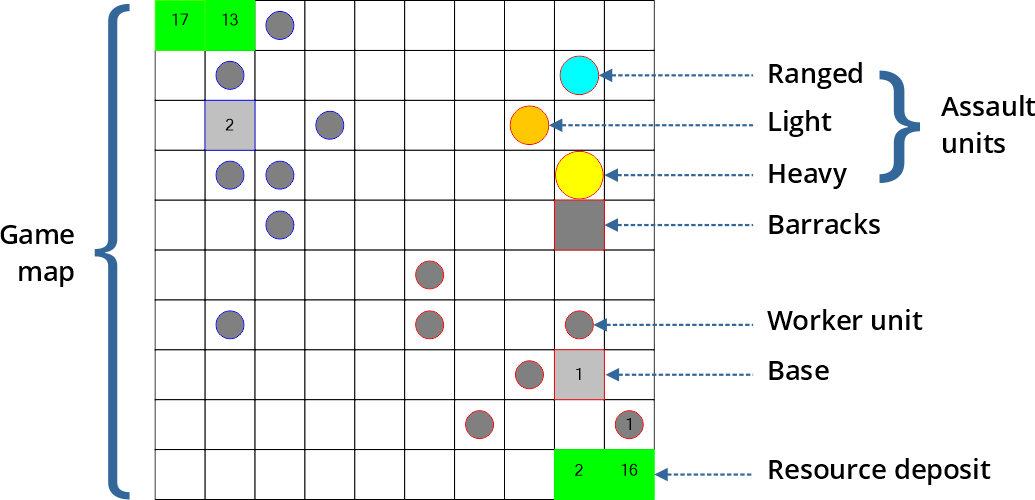
\includegraphics[scale=1]{figs/mRTS.png}
	\caption{A \mRTS{} match. The players' units can be differentiated by the color of their outline. Blue is for Player 1, and red is for Player 2. The numbers displayed over certain units indicate the amount of resources held by that unit. }
	\label{mRTSScreenshot}
\end{center}
\end{figure}

\mRTS{} represents an interesting research domain for online planning techniques, especially those requiring a forward-model. Several low-level, high-level and multi-level planning approaches were proposed in \mRTS{} as detailed in \cite{ouessai_online_2019}.

\subsection{Monte Carlo Tree Search (MCTS)}

The goal of an RTS game-playing agent is to compute the optimal player-action $a \in A$, for each decision cycle $t$, where the agent is able to act. The successive, computed player-actions constitute a plan that should lead the agent to victory. Essentially, this translates to a Markov decision process (MDP) under tight computation budget, and high search-space dimensionality constraints. MCTS is a sampling-based search framework applicable to MDPs with large decision spaces, unapproachable to systematic search techniques. MCTS relies on the execution of a large number of Monte Carlo simulations to estimate the value of actions, sampled from the search space following a tree-policy. The MCTS algorithm iteratively constructs a game tree by executing a 4-step process at each iteration. The algorithm can be halted anytime to obtain a decision. An MCTS iteration proceeds as follows : 

\begin{enumerate}
\item Selection : Select a node with unexplored children, following a tree policy.
\item Expansion : Expand the selected node by creating and attaching a new child node.
\item Simulation : Start a simulation (playout) from the new node, following a playout policy.
\item Backpropagation : Backpropagate the simulation's results starting from the new node up to the root node, updating all the intermediary nodes' statistics (visit count and value).
\end{enumerate}

The most visited decision is usually the one returned. Given enough computation budget and a proper exploration / exploitation equilibrium in the tree policy, MCTS is guaranteed to find the minimax solution, in the limits. The most popular MCTS implementation, UCT (Upper Confidence bounds for Trees), uses UCB1 formula as a tree policy, treating the selection phase as a multi-armed bandit (MAB) problem. Although remarkably successful in Go, UCT does not perform as well in RTS games, due to the rapid growth in the branching factor, with the increase in the unit count. NaïveMCTS was specifically designed to address the combinatorial search space in RTS games, by formulating the selection phase as a combinatorial MAB (CMAB). Additionally, NaïveMCTS employs a naïve sampling approach that relies on a naïve assumption considering the reward estimate of a player-action as the sum of the reward estimates of the underlying unit-actions. In our experiments, we used both UCT and NaïveMCTS as the base search algorithms for our pruning approach.

% Writing ...

\section{Related Works}

\subsection{Search Space Reduction}

Dealing with the enormous RTS decision space in the context of MCTS is an open problem, continuously receiving contributions. By treating the selection phase as a CMAB, NaïveMCTS effectively adapts MCTS to combinatorial search spaces, nevertheless, the decision space remains the same, and the algorithm still suffers from the high dimensionality. Downsizing the search space's dimensionality is usually done through action abstraction or machine learning.

Abstracting the search space, by means of expert-authored scripts, is an effective way to considerably reduce the branching factor. Instead of searching in the whole low-level player-actions space, Justesen et al \cite{justesen_script-_2014} adapted UCT to search in the space of player-actions suggested by scripts. NaïveMCTS was also adapted the same way by Moraes et al \cite{moraes_action_2018}, with the incorporation of asymmetric abstraction \cite{moraes_asymmetric_2018}, allowing multi-script and multi-level search. Puppet Search \cite{barriga_puppet_2015} employs UCT to search in the space of choice points, inserted into scripts. Guided NaïveMCTS (GNS) \cite{yang_guiding_2019} uses scripts to bias the selection phase towards considering scripted actions first. Several other search algorithms were also used in combination with action abstraction, such as local search in Portfolio Greedy Search (PGS) \cite{churchill_portfolio_2013}, and minimax in AHTN \cite{ontanon_adversarial_2015}.

Techniques that rely on machine learning try to learn a tree policy, from expert traces, that nudges the selection phase towards more promising expert actions. AlphaGo \cite{silver_mastering_2016} employs a CNN-based policy network, learned from a large dataset of expert Go replays. Ontañón introduced InformedMCTS in \mRTS{}, which makes use of a learned Bayesian model, to inform the selection phase of MCTS. Yang and Ontañón \cite{yang_extracting_2019} later demonstrated the effectiveness of C4.5 classifier for such tasks, due to its speed and accuracy.

\subsection{Move Pruning}

If we adjust our perspective, the aforementioned approaches can all be regarded as move pruning approaches \cite{yang_integrating_2020}. By focusing on a set of promising, expert-based player-actions, theses approaches effectively prune the search space of all the remaining player-actions, significantly reducing the branching factor. Regardless, such a practice can also be unsafe and prone to exploitation, due to the coarser player-actions considered, resulting in a loss of tactical performance. To address this issue, several approaches combining low- and high-level search have emerged, such as \cite{barriga_combining_2017}, \cite{neufeld_hybrid_2019} and \cite{moraes_action_2018}.

Directly pruning player-actions, responsible for weak playing strength, can be an alternative approach towards focusing search on promising actions, without compromising tactical strength. In the context Chess \cite{heinz_adaptive_1999} and Shogi \cite{hoki_efficiency_2012}, $\alpha\beta$ search was enhanced by several forward pruning methods, such as Null-move pruning and futility pruning, that reduce the branching factor by removing statistically weak moves. In Go, a domain-dependent pruning approach was implemented in UCT \cite{huang_pruning_2010-1}, exploiting territory information. Similar MCTS improvements were applied in Hex \cite{arneson_monte_2010-1}, Havannah \cite{dugueperoux_pruning_2016} and DeadEnd \cite{he_game_2008-1}. In video-games, Sephton et al \cite{sephton_heuristic_2014} also enhanced MCTS by applying a knowledge-based move pruning approach for the strategic card game, Lords of War. In this paper we apply a domain-dependent hard-pruning approach, for MCTS agents in RTS games, targeting a specific type of player-actions.

\section{Move Pruning}

We propose to act directly on the decision space, and hard-prune a portion of decisions we deem irrelevant and/or detrimental to the performance of MCTS. By doing so, MCTS will be freed from sampling those decisions and simulating their outcomes, and the computation budget gained will be utilized to focus on, hopefully, more relevant and significant decisions. Consequentially, the playing strength and scalability of MCTS should be improved.

As a first attempt, we chose to focus on player-actions having the highest chance of misleading search, and negatively impacting the playing strength. Out of these player-actions, we believe Inactive Player-Actions (IPAs) naturally come first. Thus, we implemented a number of pruning approaches that keep a predefined amount (fixed or relative) of those player-actions, and prune the remaining. We will briefly discuss the structure of RTS player-actions, and then define IPAs.

\subsection{Unit-Actions and Player-Actions}

In a typical RTS game, each unit type can execute a distinct set of actions, known as unit-actions. Table \ref{unitActionsTable} enumerates the unit-action types executable by each unit type in \mRTS{}. The Worker unit type is clearly the most versatile type, followed by assault units (Light, Ranged, Heavy), then structures (Base, Barracks). The attributes of each unit-type define how a unit-action is executed. For instance, the damage attribute governs how much damage a unit-type causes when executing the Attack unit-action, thus, each unit type is unique in the way it behaves, even for shared unit-actions. All unit-action types, except Wait, require a positional argument to define where, or on whom the action should be taken. The Wait unit-action type requires a numeric argument determining how many cycles the unit should remain idle. Wait is also the single unit-action type executable by all unit types.

\begin{table}[!h]
\renewcommand{\arraystretch}{1.3}
\caption{The unit-action types available for each unit type in \mRTS{}}
\label{unitActionsTable}
\centering
\begin{tabular}{|c|c|c|c|c|c|c|}
\cline{2-7}
\multicolumn{1}{c|}{} & Move & Attack & Harvest & Return & Produce & Wait \\
\hline
Worker   & $\bullet$ & $\bullet$ & $\bullet$ & $\bullet$ & $\bullet$ & $\bullet$ \\
%\hline
Light    & $\bullet$ & $\bullet$ & & & & $\bullet$ \\
%\hline
Ranged   & $\bullet$ & $\bullet$ & & & & $\bullet$ \\
%\hline
Heavy    & $\bullet$ & $\bullet$ & & & & $\bullet$ \\
%\hline
Base     & & & & & $\bullet$ & $\bullet$ \\
%\hline
Barracks & & & & & $\bullet$ & $\bullet$ \\
\hline
\end{tabular}
\end{table}

A player-action $p \in A$, issued to $n$ units at a given game cycle, can be regarded as a tuple, where $p = (a_1, a_2, \dots, a_n)$, and each component $a_i$ represents a unit-action issued by the player, to the same-indexed unit. Assuming that each unit is assigned a valid and legal unit-action and given the average number of unit-actions available to each unit, $m$, the number of all possible player-actions, or the branching factor, $b$, can be estimated as $b = m^n$. We seek to lower $b$, by finding ways to decrease $m$ without negatively impacting the playing strength.

\subsection{Inactive Player-Actions}

We define an Inactive Player-Action (IPA) as a player-action having at least one Wait (inactive, idle, no-op) unit-action as a component. Being the most prevalent, non-critical unit-action, Wait unit-actions make for a good pruning target. A Wait unit-action is always an available option to any unit, regardless the situation, hence, it strongly participates in the inflation of the search space. Nevertheless, Wait unit-actions can be useful for a unit in the following situations :
\begin{itemize}
\item Trapped unit : no active unit-action possible. i.e. the unit is caught in a situation where all possible unit-actions are illegal. Waiting for a number of cycles is the only option to choose in hopes the situation resolves itself.
\item Anticipating unit : the unit anticipates for a chance to execute a high value unit-action. Here, the unit excepts a sub-optimal action by an opponent unit and chooses to Wait in anticipation for it in order to later execute an advantageous action. This behaviour is frequently observed in tactical skirmishes.
\end{itemize}
Although mildly useful, Wait unit-actions can also have a devastating effect on playing strength if improperly chosen. According to our observation, it is not unlikely for a search-based agent to assign a Wait unit-action to a unit in a situation where better options exist. In such cases, doing nothing is the worst decision possible. We identify three situations where Waiting cannot be a sound decision :
\begin{itemize}
\item Waiting in front of opportunity : Here, the unit is able to seize an immediate opportunity, such as Harvest resources, Return harvested resources, or safely remove an opponent unit, instead, the unit is assigned Wait.
\item Waiting in face of danger : The unit is facing an immediate danger, and holds the necessary options to avoid it, but instead, it is assigned a Wait unit-action.
\item Waiting randomly : Instead of all the safe options available, the unit is assigned a Wait unit-action.
\end{itemize}


\subsection{Pruning Techniques}
% not possible to identify 
\section{Experimentation Results}

\subsection{Parameter Tuning}

% WIP

\begin{figure*}[!h]
\begin{center}
	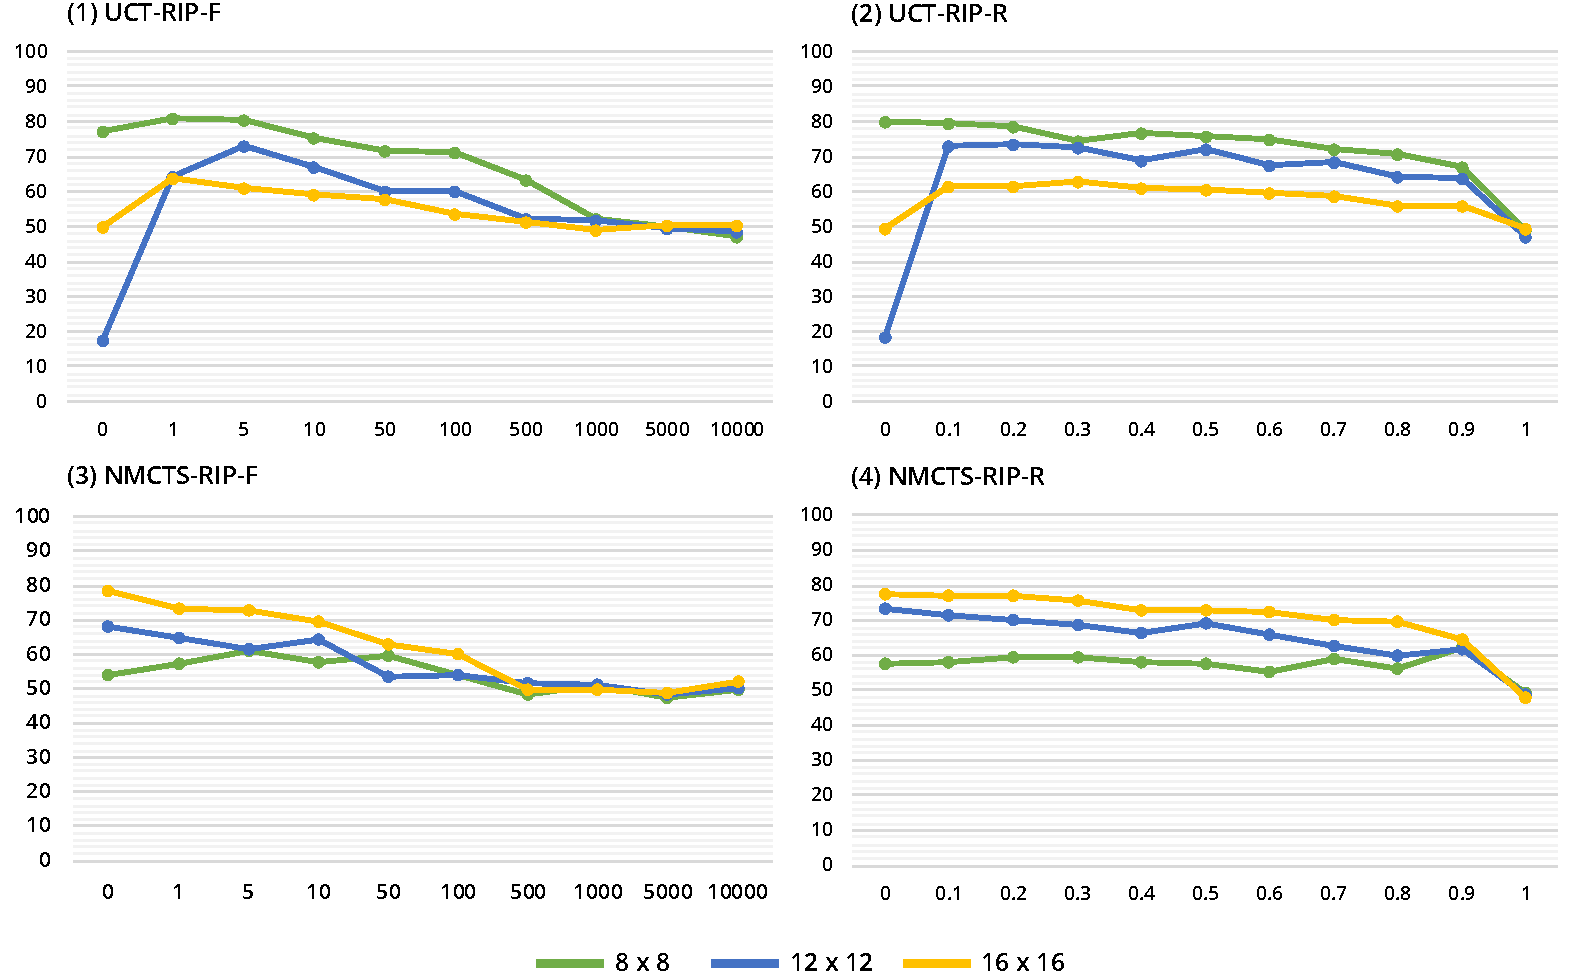
\includegraphics[width=0.8\textwidth]{figs/PT.pdf}
	\caption{UCT-RIP-F performance against UCT}
	\label{PT}
\end{center}
\end{figure*}

\subsection{Best Pruning Approach}

\subsection{Tournament}

\section{Conclusion}

\bibliographystyle{IEEEtranS}
\bibliography{library}

\end{document}
